\label{chapter:data}

Este capítulo tem como objetivo explorar características do tráfego e caracterizar do conjunto de dados utilizado nesse trabalho. Primeiramente, são explicadas as características do tráfego e como ele pode ser modelado. Em seguida, é explicitado como os dados que serão utilizados no capítulo \ref{chapter:methodology} foram adquiridos, assim como suas características. 

\section{Tráfego}

É importante salientar que o tráfego é afetado por diversos fatores, entre eles: temporais, espaciais e exógenos. Entre os fatores temporais estão, por exemplo, o horário do expediente dos trabalhadores que possuem veículos, ou se é ou não final de semana. Entre os fatores espaciais estão, por exemplo, como a malha rodoviária se distribui em uma localização, ou a quantidade de empresas em uma área. Já fatores exógenos são externos as características do tráfego, por exemplo, acidentes que possam vir a ocorrer, ou meteorologia do dia. Sendo assim, modelos de previsões podem ter desempenhos diferentes dependendo de onde e quando os dados forem coletados.

Dessa forma, é comum na literatura optar-se por usar apenas dados com fatores espaciais e temporais \cite{lana_2018}. Ao se desconsiderar os fatores exógenos, é feita uma suposição de que exista uma tendência no fluxo que pode ser prevista e que, embora as variáveis aleatórias possam afetar o fluxo, elas não afetam o bastante para mudar a tendência no longo prazo. Seguindo a literatura, esse trabalho utilizará variáveis temporais e espaciais. 

Além disso, segundo Zainab Abbas et. al. \cite{Zainab_2018}, o tráfego pode ser interpretado de maneiras diferentes. Pode ser interpretado como a quantidade de veículos que passaram por um ponto em um determinado intervalo de tempo, o fluxo de veículos. Também pode ser interpretado como o fluxo dividido pela média de velocidade dos veículos em um certo espaço de tempo, a densidade. Ou pode ser interpretado como uma média de velocidade em um intervalo de tempo, a velocidade média.

\section{Caracterização do Conjunto de Dados}

Esta seção almeja demonstrar o formato dos dados, assim como a maneira na qual eles foram adquiridos. São apresentadas tabelas que mostram as colunas exatas e imagens aéreas dos cruzamentos, onde estão instalados os fiscalizadores responsáveis pela captura de informações.

\subsection{Aquisição dos Dados}

Os dados\footnote{http://bit.ly/processed-data-2l5MaAG} provêm de dois cruzamentos na avenida Hélio Prates que pode ser vista na Figura \ref{figure:helio}. Esta cruza Taguatinga e Ceilândia, que são duas cidades satélites do \acrshort{DF}. Estes dados foram coletados por fiscalizadores eletrônicos localizados nos cruzamentos e foram fornecidos pelo \acrshort{DETRAN}\footnote{http://www.detran.df.gov.br/} do \acrshort{DF}. Neste conjunto de dados estão inclusos registros de todos os veículos que passaram pelo local nos meses de maio a julho de 2016 em forma de uma série temporal. Mais especificamente, do primeiro dia de maio ao último de julho de 2016, totalizando 13 semanas e 1 dia, 92 dias. Vale notar que esses dados foram escolhidos devido a sua disponibilidade.

\begin{table}[htbp]
    \begin{tabular}{ccccccc}
    \toprule
    \multicolumn{1}{l}{\textbf{Id Equip.}} & \multicolumn{1}{l}{\textbf{Data}} & \multicolumn{1}{l}{\textbf{Hora}} & \multicolumn{1}{l}{\textbf{Faixa}} & \multicolumn{1}{l}{\textbf{km/h}} & \multicolumn{1}{l}{\textbf{km/h Max}} & \multicolumn{1}{l}{\textbf{Tamanho}} \\ 
    \midrule
        RSI128 & 2016/05/01 & 00:00:09 & 1 & 20 & 60 & 0.0 \\
    \midrule
    RSI131 & 2016/05/01 & 00:00:09 & 2 & 45 & 60 & 1.1 \\
    \midrule
    RSI132 & 2016/05/01 & 00:00:09 & 1 & 40 & 60 & 0.0 \\
    \midrule
    RSI131 & 2016/05/01 & 00:00:10 & 1 & 35 & 60 & 0.5 \\
    \midrule 
    RSI129 & 2016/05/01 & 00:00:12 & 1 & 35 & 60 & 0.0 \\
    \midrule
    RSI131 & 2016/05/01 & 00:00:13 & 1 & 43 & 60 & 1.0 \\
    \midrule
    RSI131 & 2016/05/01 & 00:00:14 & 1 & 35 & 60 & 1.2 \\
    \midrule
    RSI128 & 2016/05/01 & 00:00:18 & 1 & 32 & 60 & 0.0 \\
    \midrule
    RSI131 & 2016/05/01 & 00:00:19 & 2 & 41 & 60 & 1.1 \\
    \midrule
    RSI129 & 2016/05/01 & 00:00:20 & 1 & 37 & 60 & 0.0 \\
    \midrule
    RSI131 & 2016/05/01 & 00:00:22 & 1 & 49 & 60 & 1.5 \\
    \midrule
    RSI018 & 2016/05/01 & 00:00:36 & 2 & 47 & 60 & 0.0 \\
    \midrule
    RSI018 & 2016/05/01 & 00:00:43 & 2 & 40 & 60 & 0.0 \\
    \midrule
    RSI018 & 2016/05/01 & 00:00:45 & 2 & 37 & 60 & 0.0 \\
    \midrule
    RSI033 & 2016/05/01 & 00:00:52 & 2 & 17 & 60 & 0.0 \\
    \bottomrule
    \end{tabular}
    \label{table:data}
    \caption{Exemplo dos dados recebidos coletados pelo \acrshort{DETRAN}}
\end{table}

\subsection{Características dos Dados}

Quanto as características das colunas, o conjunto de dados possui tanto colunas quantitativas quanto qualitativas. Só existe uma coluna qualitativa, \texttt{Id Equipamento}, sendo ela ordinal, pois em seu nome ocorre uma numeração. Todas as outras colunas são quantitativas, sendo a de tamanho a única contínua e o resto discreto. Porém a coluna de \texttt{km/h Max} tem seu valor constante constante.  Os registros são de 8 sensores com um total de 10.801.781 registros de veículos. Vale notar que nem todos os sensores estão localizados na Avenida Hélio Prates, alguns estão localizados na avenidas que cruzam a mesma. Além disso, a quantidade de registros por sensor não distribuídos igualmente:

\begin{itemize}
    \item \textbf{RSI033:} 2.382.754 registros de veículos
    \item \textbf{RSI032:} 2.117.820 registros de veículos
    \item \textbf{RSI018:} 2.029.559 registros de veículos
    \item \textbf{RSI017:} 1.686.900 registros de veículos
    \item \textbf{RSI131:} 816.219 registros de veículos
    \item \textbf{RSI132:} 652.998 registros de veículos
    \item \textbf{RSI129:} 578.652 registros de veículos
    \item \textbf{RSI128:} 536.879 registros de veículos
\end{itemize}

Os sensores contém dados de um mesmo período, sendo assim, quanto maior a quantidade de veículos mais intenso foi o tráfego. Os quatro sensores com maior fluxo pertencem a via principal, assim como pode ser visto na Figura \ref{figure:helio_cruzamento_1} e \ref{figure:helio_cruzamento_2}. Vale salientar que não foram encontrados atributos incompletos ou nulos. Porém uma das colunas possui dados inconsistentes com a realidade. Isso acontece pois, como pode ser visto na Tabela \ref{table:data} existem veículos com tamanho 0, o que é impossível. Por último, mas não menos importante, também deve-se notar que os fiscalizadores eletrônicos utilizados ficam próximos de semáforos. Desta foram, existem momentos em que o fluxo diminui bastante, devido aos sinais vermelhos. 

\begin{figure}[htbp]
    \centering
    \includegraphics[scale=0.55,angle=90]{monography/img/maps/avenida_helio_prates.png}
    \label{figure:helio}
    \caption[Visão Espacial da Avenida Hélio Prates Provindos do Apple Maps]{Visão Espacial da Avenida Hélio Prates Provindos do Apple Maps}
\end{figure}

\begin{figure}[htpb]
    \centering
    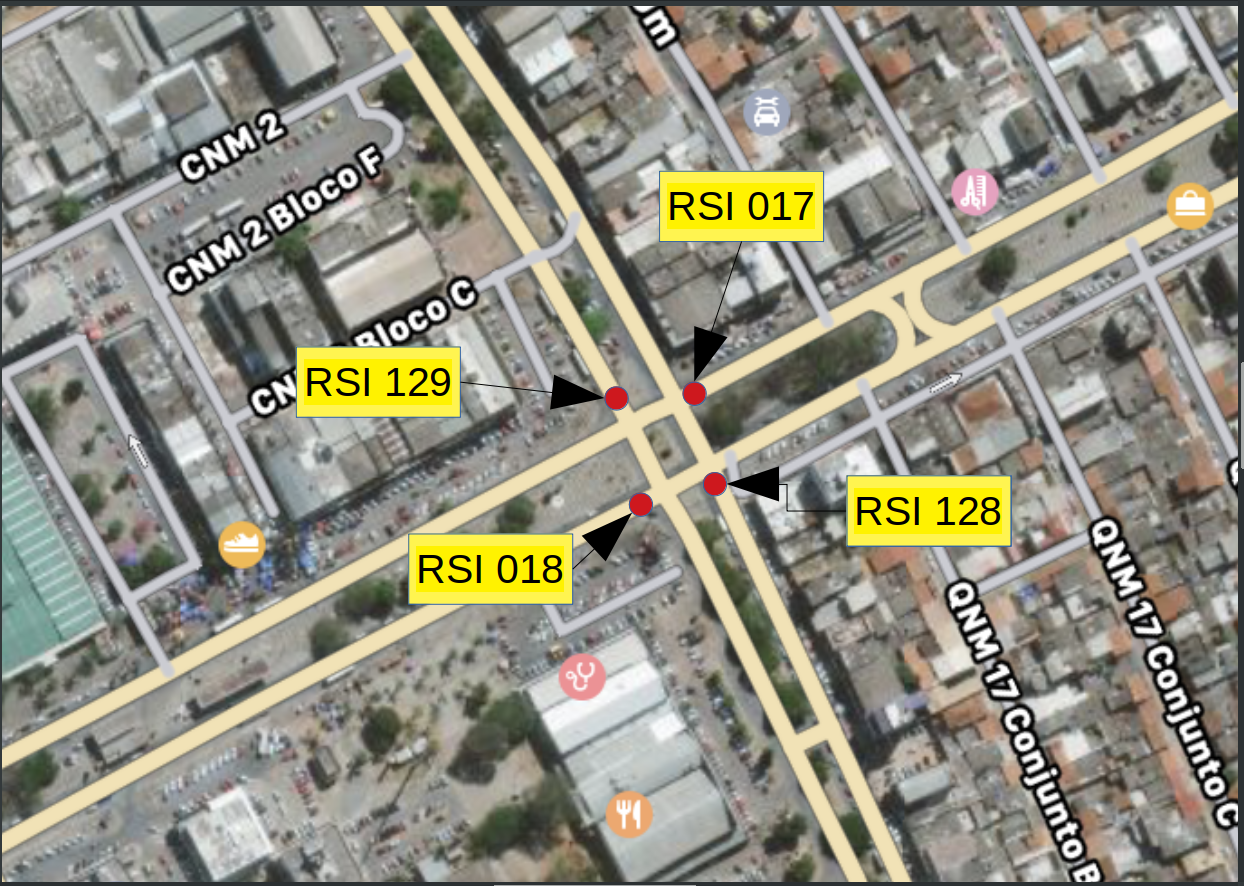
\includegraphics[scale=0.3]{monography/img/maps/crossing_1.png}
    \label{figure:helio_cruzamento_1}
    \caption[Visão Espacial do Cruzamento referente aos sensores \textbf{RSI128}, \textbf{RSI129}, \textbf{RSI017} e \textbf{RSI018}]{Visão Espacial do Cruzamento referente aos sensores \textbf{RSI128}, \textbf{RSI129}, \textbf{RSI017} e \textbf{RSI018}}
\end{figure}

\begin{figure}[htbp]
    \centering
    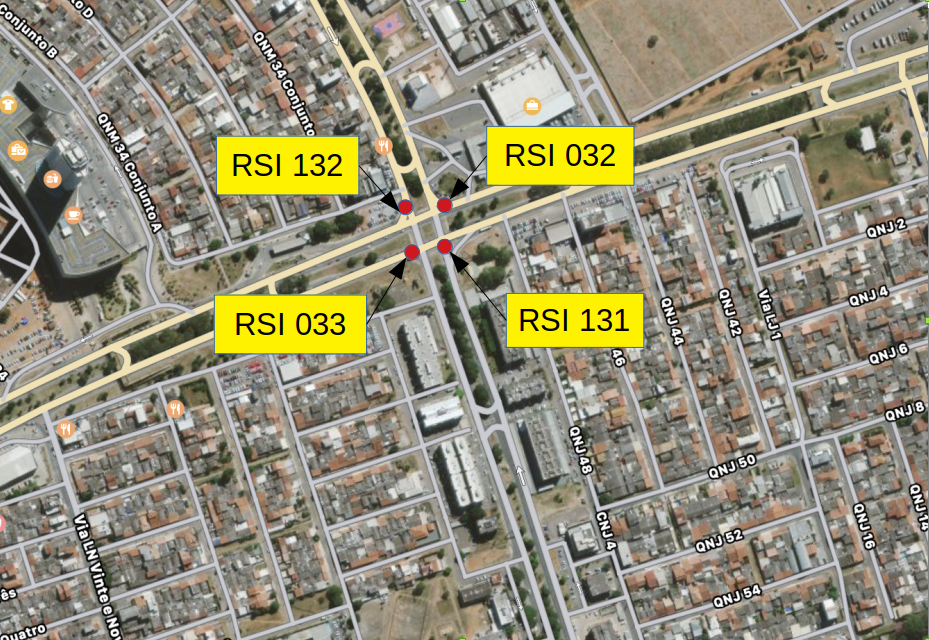
\includegraphics[scale=0.4]{monography/img/maps/crossing_2.png}
    \label{figure:helio_cruzamento_2}
    \caption[Visão Espacial do Cruzamento referente aos sensores \textbf{RSI131}, \textbf{RSI132}, \textbf{RSI032} e \textbf{RSI033}]{Visão Espacial do Cruzamento referente aos sensores \textbf{RSI131}, \textbf{RSI132}, \textbf{RSI032} e \textbf{RSI033}}
\end{figure}

\subsection{Escopo dos Dados}

O conjunto de dados provém de uma só cidade, recolhidos de sensores instalados em locais específicos e por apenas 3 meses. Logo, os resultados podem não ser os mesmos quando a metodologia for utilizada em outras localidades ou outros meses. O modo como os motoristas dirigem e como as vias são feitas também vão influenciar. Para a previsão perfeita seriam necessárias muitas variáveis, as quais não estão disponíveis.

Além disso, existem casos e cenários que os fiscalizadores eletrônicos não são capazes de registrar. Entre eles estão:

\begin{itemize}
    \item Falhas no equipamento
    \item Bloqueio em vias
    \item Acidentes de trânsitos
    \item Greves, movimentações e eventos
    \item Incapacidade de registrar uma velocidade média do veículo ao longo da via (visto que não há registro de placas)
    \item Carros transitando em velocidades ilegais na falta de presença de fiscalização eletrônica.
\end{itemize}
